\documentclass{article}

\usepackage[margin=3cm]{geometry}
\usepackage{amsmath, amssymb, amsthm}
\usepackage{url}
\usepackage{graphicx}
\usepackage{eqlist}
\usepackage{uri}
\urisetup{doipre={https://doi.org/}}
\usepackage{natbib}
\usepackage{siunitx}
\usepackage{pythonhighlight}
\usepackage{comment}
\usepackage{caption}
\usepackage{tabularx}
\usepackage{tikz}
\usepackage[font={small}, labelfont=bf]{caption}
\captionsetup{width=.7\textwidth, font=small}
\usepackage{hyperref}
\hypersetup{
    colorlinks=true,
    urlcolor=blue,
    % hidelinks=true,
    linkcolor=black,
    citecolor=black,
}
% set the float page fraction
\renewcommand{\floatpagefraction}{.8}

% Initialize line spacing to 1.5
\linespread{1.5}

% Define \sgn function
\DeclareMathOperator{\sgn}{sgn}
\DeclareMathOperator{\real}{Re}
\DeclareMathOperator{\imag}{Im}
\DeclareMathOperator{\Ei}{Ei}
\DeclareMathOperator{\E1}{E_1}
\DeclareMathOperator{\atan2}{atan2}
% \DeclareMathOperator{\Pr}{Pr}

\title{Paddocks}

\author{Ewan Short}

\date{\today}

\begin{document}

\maketitle

\noindent You're building a farm, and need to plan some paddocks. You've ordered fences from Amazon, and each piece of fence is exactly one meter long. We write ``one meter'' as \SI{1}{\meter} for short. We will use our graph paper to plan our paddocks. Imagine that each square of your \SI{1}{\centi\meter} by \SI{1}{\centi\meter} graph paper corresponds to $\SI{1}{\meter}$ by $\SI{1}{\meter}$ in the real world. Pretend that Barnaby Joyce has passed a law that all paddocks must be rectangles. Then on your graph paper, we can draw our paddocks as rectangles following the grid lines. Figure \ref{Fig:example_paddocks} shows some example paddocks. The first paddock has sides of 8 meters and 6 meters, and covers exactly 48 square meters (count the squares on the graph paper to check this!) 

\newcommand{\paddock}[4]{
    % #1,#2 = bottom-left corner
    % #3,#4 = width, height (in meters)    
    \draw[blue, thick] (#1,#2) rectangle (#1+#3,#2+#4);
    \pgfmathparse{int(#3)}
    \let\widthlabel\pgfmathresult
    \pgfmathparse{int(#4)}
    \let\heightlabel\pgfmathresult
    \pgfmathparse{int(\heightlabel*\widthlabel)}
    \let\arealabel\pgfmathresult
    \node[below=2pt] at (#1+#3/2,#2) {\widthlabel\ m};
    \node[left=2pt] at (#1,#2+#4/2) {\heightlabel\ m};
    \node at (#1+#3/2,#2+#4/2) {\arealabel\ m$^2$};
}

\begin{figure}[ht]
    \centering
    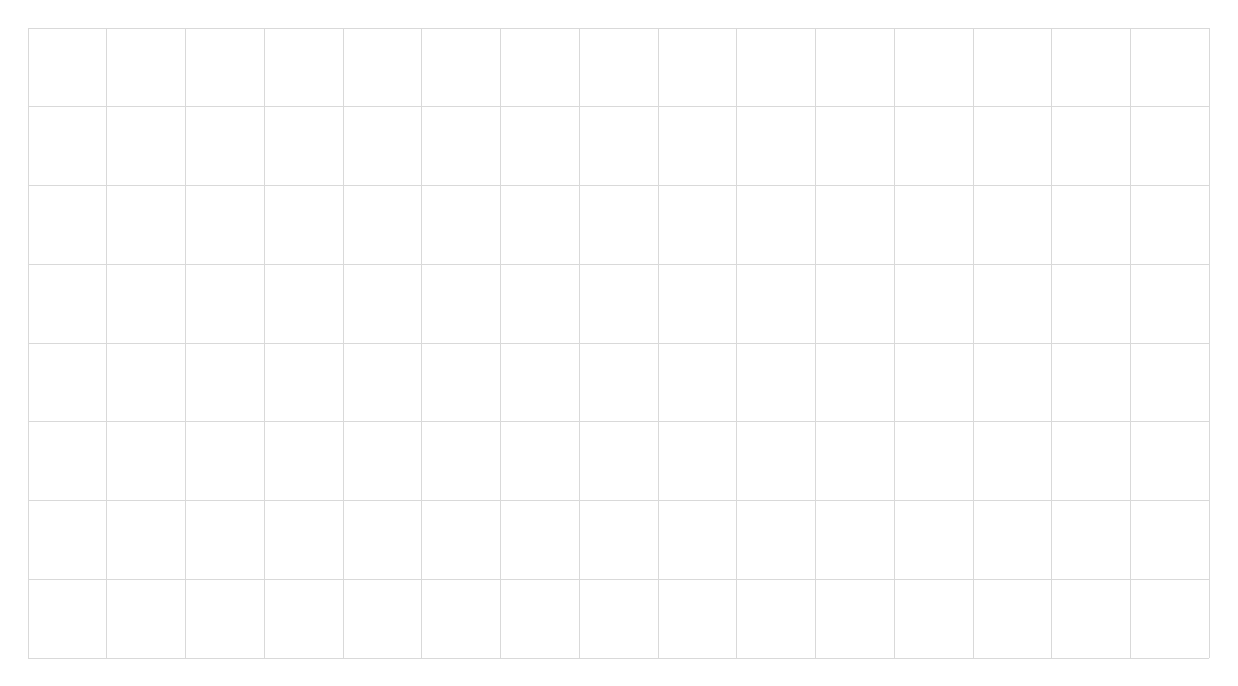
\begin{tikzpicture}
        % Light grid (graph paper background)
        \draw[step=1cm, gray!30, very thin] (0, 0) grid (15, 8);
        \paddock{1}{1}{8}{6}
        \paddock{11}{2}{3}{2}
    \end{tikzpicture}
    \caption{Some example paddocks on graph paper.}
    \label{Fig:example_paddocks}
\end{figure}

\section{Times-Table Paddocks}
\noindent To get started, let's practice multiplication by creating some paddocks. I like the numbers 3 and 7, so let's visualize $3\times 7$ as a paddock. The paddocks in Fig.~\ref{Fig:three_by_seven} have sides of \SI{3}{\meter} and \SI{7}{\meter}, and cover and area of \SI{21}{\meter\squared}, so $3\times 7 = 21$. Remember also that
$$3\times 7 = \underbrace{7 + 7 + 7}_{\text{3 lots of 7}},$$ 
so to show this I've drawn lines on each paddock to separate out 3 blocks of 7 in different ways.

\begin{figure}[ht]
    \centering
    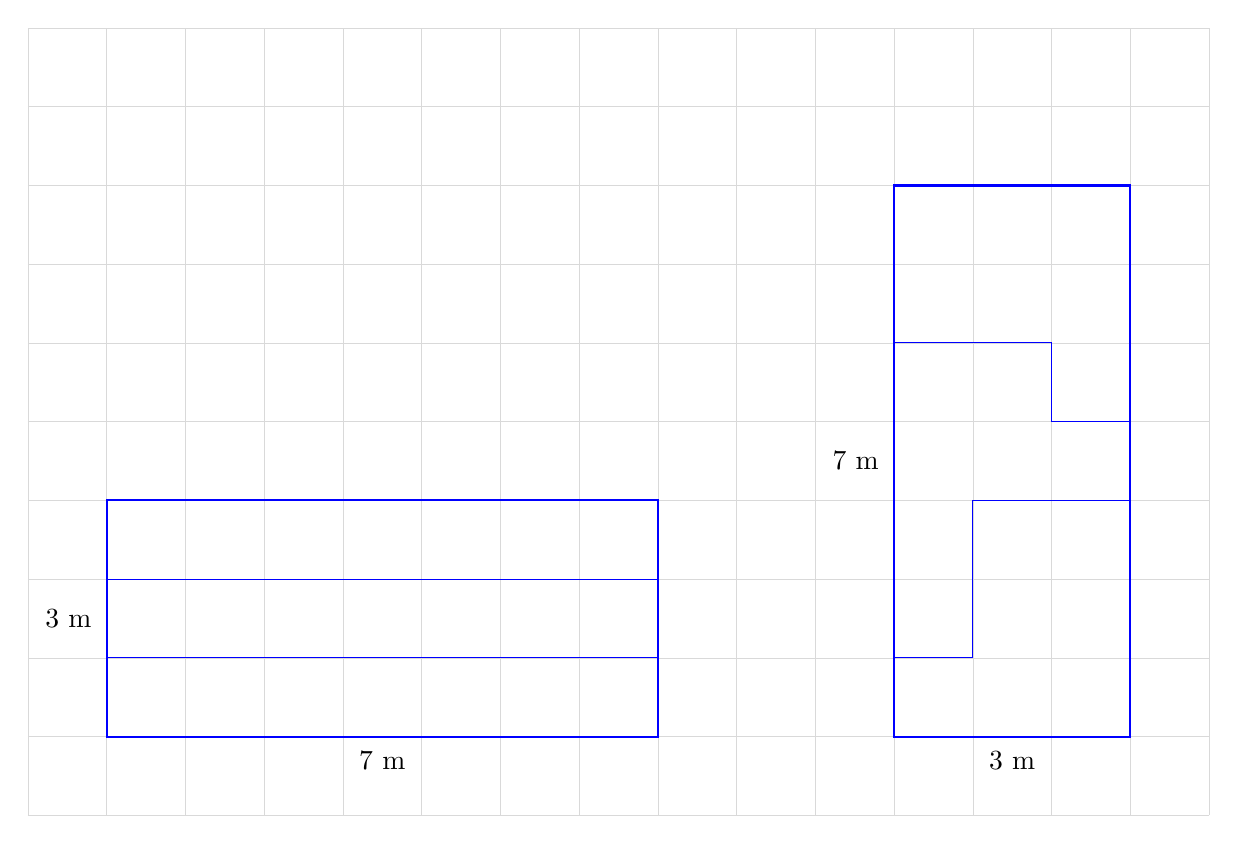
\begin{tikzpicture}
        % Light grid (graph paper background)
        \draw[step=1cm, gray!30, very thin] (0, 0) grid (15, 10);
        
        % First paddock: 3×7 (landscape orientation)
        % Draw horizontal lines separating the rows of the paddock
        \draw[blue] (1,2) -- (8,2);
        \draw[blue] (1,3) -- (8,3);

        % Draw outer border
        \draw[blue, thick] (1,1) rectangle (8,4);
        
        % Add labels
        \node[below=2pt] at (4.5,1) {7 m};
        \node[left=2pt] at (1,2.5) {3 m};
        
        % Second paddock: 7×3 (portrait orientation)
        % Draw lines to separate three distinct chunks of 7 squares each
        % The rectangle is 3 wide × 7 tall = 21 squares total
        
        % Boundary between chunk 1 and chunk 2 (zigzag pattern)
        \draw[blue] (11,2) -- (12,2) -- (12,4) -- (14,4);
        
        % Boundary between chunk 2 and chunk 3 (another zigzag pattern)
        \draw[blue] (11,6) -- (13,6) -- (13,5) -- (14,5);
        
        % Draw outer border
        \draw[blue, thick] (11,1) rectangle (14,8);
        
        % Add labels
        \node[below=2pt] at (12.5,1) {3 m};
        \node[left=2pt] at (11,4.5) {7 m};
        
    \end{tikzpicture}
    \caption{Two visualizations of $3\times 7$ using paddocks.}
    \label{Fig:three_by_seven}
\end{figure}

\begin{itemize}
\item
What is your favourite number? Is there a number that is important in your culture or religion? Create some paddocks with this number as a side, work out the area, and write out the corresponding equations, like $3\times 7 =21$ in the example above.
\item
Which times-table do you find the hardest? Is there a particular multiplication you find stressful? Repeat the above exercise for the multiplications you most hate!
\end{itemize}

\section{Unique Paddocks}
Suppose we want to build a paddock with a specific area, and we want to count the number of distinct ways we can make a paddock with that area. For example, suppose we want to build a paddock with area \SI{1}{\meter\squared}. Take a look at the paddocks below in Fig.~\ref{Fig:more_example_paddocks}. Notice there is only one way to build a \SI{1}{\meter\squared} paddock with our \SI{1}{\meter} long fences - a single square on the graph paper!

For a paddock of \SI{2}{\meter\squared}, we can have either a \SI{1}{\meter} by \SI{2}{\meter} paddock, or a \SI{2}{\meter} by \SI{1}{\meter} paddock. But notice how these paddocks look pretty much the same if we rotate our graph-paper! If we shift and rotate the \SI{2}{\meter} by \SI{1}{\meter} paddock, it will look exactly like the \SI{1}{\meter} by \SI{2}{\meter} paddock! So there is once again only really one way to build a \SI{2}{\meter\squared} paddock.\footnote{If you do maths at uni you will learn about things like isomorphisms and equivalence-classes, which allow us to define precisely what we mean by ``look pretty much the same.''}

Now look at the \SI{4}{\meter\squared} paddocks in Fig.~\ref{Fig:more_example_paddocks}. We have drawn a \SI{1}{\meter} by \SI{4}{\meter} paddock, and a \SI{2}{\meter} by \SI{2}{\meter} paddock. These paddocks look very different! There is no way we can shift and rotate the \SI{1}{\meter} by \SI{4}{\meter} paddock to make it look like the \SI{2}{\meter} by \SI{2}{\meter} paddock. So there are two ways to build a \SI{4}{\meter\squared} paddock.

\begin{figure}[ht]
    \centering
    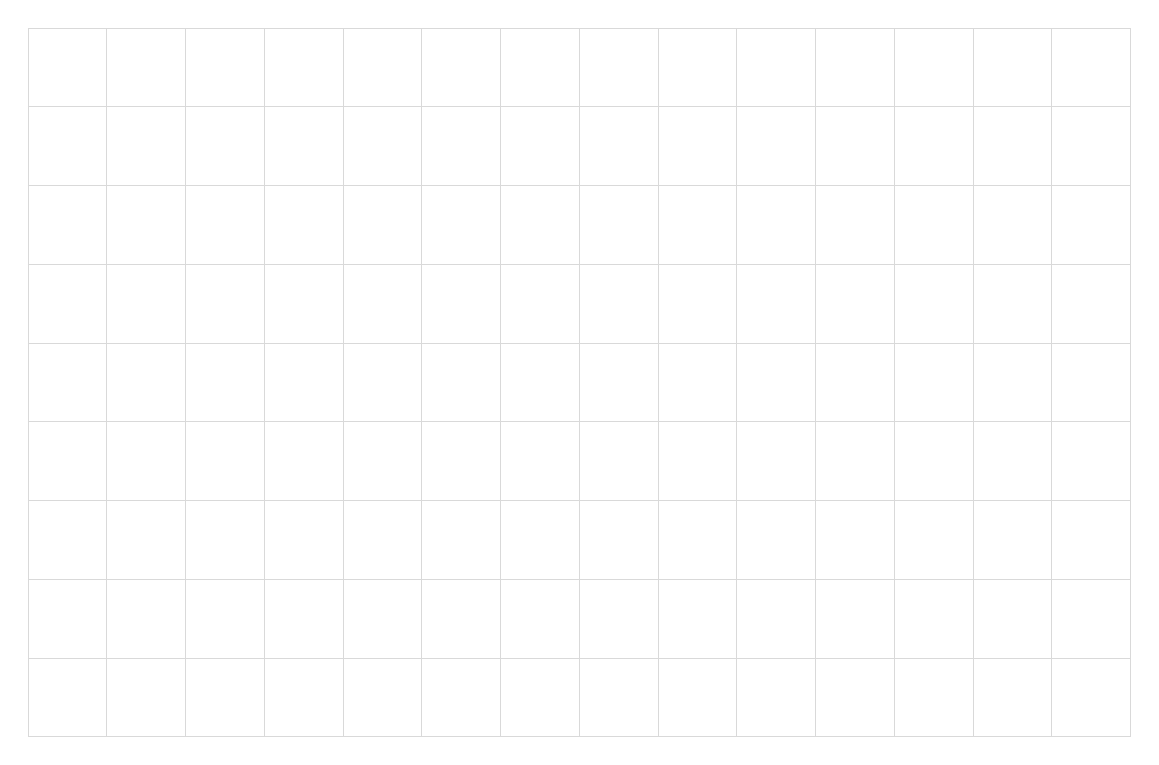
\begin{tikzpicture}
        % Light grid (graph paper background)
        \draw[step=1cm, gray!30, very thin] (0, 0) grid (14, 9);
        \paddock{2}{6}{1}{1}
        \paddock{6}{6}{1}{2}
        \paddock{10}{6}{2}{1}
        \paddock{3}{1}{1}{4}
        \paddock{9}{1}{2}{2}
    \end{tikzpicture}
    \caption{More example paddocks.}
    \label{Fig:more_example_paddocks}
\end{figure}

\begin{itemize}
    \item How many ways can we build a \SI{5}{\meter\squared} paddock?
    \item How many ways can we build a \SI{6}{\meter\squared} paddock?
    \item How many ways can we build a \SI{12}{\meter\squared} paddock?
    \item How many ways can we build a \SI{13}{\meter\squared} paddock?
    \item For each of your paddocks, write an equation expressing the area of the paddock in terms of its width and height, for example $\SI{1}{\meter}\times \SI{1}{\meter} = \SI{1}{\meter \squared}$, $\SI{1}{\meter}\times \SI{2}{\meter} = \SI{2}{\meter\squared}$, $\SI{2}{\meter}\times \SI{2}{\meter} = \SI{4}{\meter\squared}$, etc.
    \item You should now have realized that for some numbers, there is only one way to build a paddock with an area equal to that number. For these special numbers the paddocks should look long and thin. These special numbers have a name, and are very important in maths. Use your phone or computer to try to work out what these special numbers are called!
    \item How many ways can we build a \SI{3318308475676071413}{\meter\squared} paddock?
\end{itemize}

\section{Animal Storage}
We now need to build some paddocks to put our animals in. As listed in Table \ref{Tab:animals}, our different animals need different amounts of space in our paddocks, and some animals will eat others if placed beside them. As the animal names suggest, we will use fruit/nuts/chocolate to represent our animals. 

\begin{table}[ht]
    \centering
    \begin{tabular}{|c|c|c|}
        \hline
        \textbf{Animal} & \textbf{Area Needed} & \textbf{Eats} \\
        \hline
        Choco-dile & \SI{6}{\meter} by \SI{3}{\meter} & Date-opotamus, Almond-vark, other Choco-dile \\
        Date-opotamus & \SI{4}{\meter} by \SI{3}{\meter} & Almond-vark \\
        Almond-vark & \SI{3}{\meter} by \SI{2}{\meter} & Curr-ant \\
        Curr-ant & \SI{1}{\meter} by \SI{1}{\meter} & - \\
        \hline
    \end{tabular}
    \caption{Summary of our animals.}
    \label{Tab:animals}
\end{table}

Figure \ref{Fig:food_animals} shows a picture of our animals.\footnote{I used Google Gemini to make these pictures. If math is getting stressful, draw your own food animals!} Draw arrows on this picture to illustrate the food chain. For example, you should draw an arrow from the Curr-ant to the Almond-vark, as Almond-varks eat Curr-ants, and a loopy arrow from the Choco-dile to itself, as Choco-diles eat other Choco-diles.\footnote{Diagrams of objects with arrows connecting them are called ``networks'', ``directed graphs'' or just ``graphs". These special graphs are very important in mathematics and life, powering A.I. chatbots, the human brain, Google's search algorithm, traffic flows, epidemics, and many other things!}

\begin{figure}[h]
    \centering
    \includegraphics[width=.75\linewidth]{food_animals.jpg}
    \caption{Our animals.}
    \label{Fig:food_animals}
\end{figure}

Next, plan your paddock under the following constraints. 
\begin{enumerate}
\item
You have exactly 36 fences.
\item
You cannot put animals next to other animals that will eat them (but touching at corners is ok!)
\item
You're only allowed at most two Choco-diles in your paddock.
\end{enumerate} 
An example paddock plan is shown in Fig.~\ref{Fig:animal_paddock} below. Make sure your own paddock is different from the one in Fig.~\ref{Fig:animal_paddock}!
\begin{figure}[ht]
    \centering
    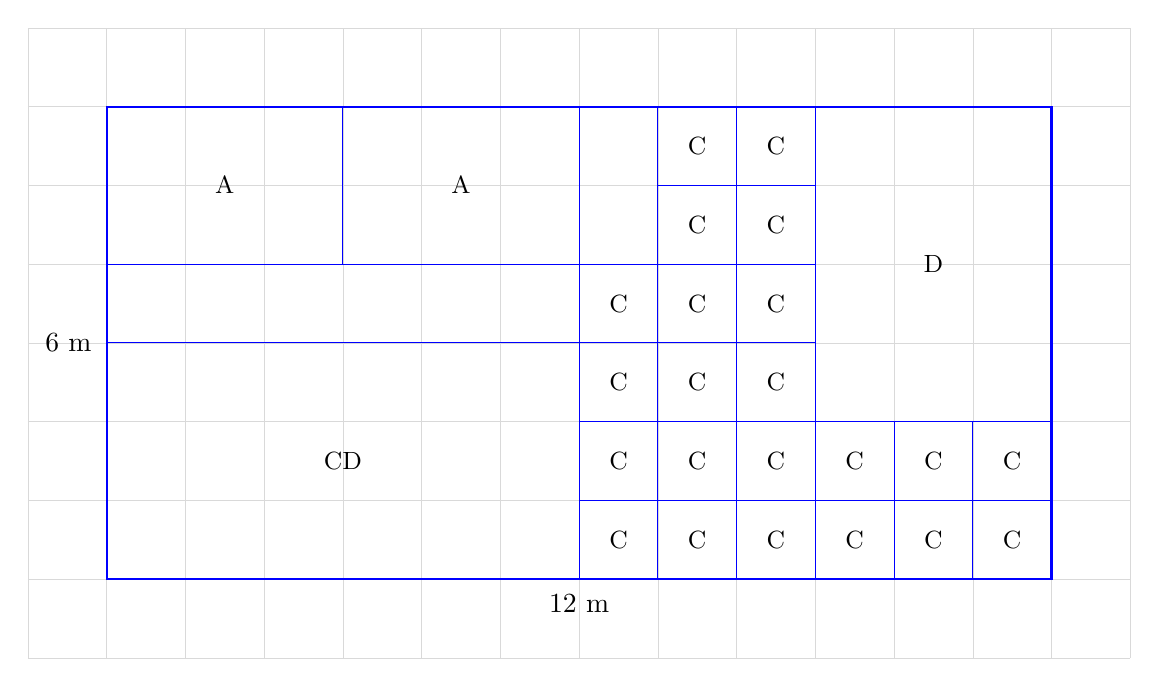
\begin{tikzpicture}
        % Light grid (graph paper background)
        \draw[step=1cm, gray!30, very thin] (0, 0) grid (14, 8);

        % Choco-dile
        \draw[blue] (1, 1) rectangle (7, 4);
        \node[font=\small] at (4, 2.5) {CD};
        
        % Curr-ant
        \draw[blue] (7, 4) rectangle (8, 5);
        \node[font=\small] at (7.5, 4.5) {C};
        \draw[blue] (7, 3) rectangle (8, 4);
        \node[font=\small] at (7.5, 3.5) {C};
        \draw[blue] (7, 2) rectangle (8, 3);
        \node[font=\small] at (7.5, 2.5) {C};
        \draw[blue] (7, 1) rectangle (8, 2);
        \node[font=\small] at (7.5, 1.5) {C};
        \draw[blue] (8, 1) rectangle (9, 2);
        \node[font=\small] at (8.5, 1.5) {C};
        \draw[blue] (9, 1) rectangle (10, 2);
        \node[font=\small] at (9.5, 1.5) {C};
        \draw[blue] (8, 2) rectangle (9, 3);
        \node[font=\small] at (8.5, 2.5) {C};
        \draw[blue] (9, 2) rectangle (10, 3);
        \node[font=\small] at (9.5, 2.5) {C};
        \draw[blue] (8, 3) rectangle (9, 4);
        \node[font=\small] at (8.5, 3.5) {C};
        \draw[blue] (9, 3) rectangle (10, 4);
        \node[font=\small] at (9.5, 3.5) {C};
        \draw[blue] (8, 4) rectangle (9, 5);
        \node[font=\small] at (8.5, 4.5) {C};
        \draw[blue] (9, 4) rectangle (10, 5);
        \node[font=\small] at (9.5, 4.5) {C};
        \draw[blue] (8, 5) rectangle (9, 6);
        \node[font=\small] at (8.5, 5.5) {C};
        \draw[blue] (9, 5) rectangle (10, 6);
        \node[font=\small] at (9.5, 5.5) {C};
        \draw[blue] (8, 6) rectangle (9, 7);
        \node[font=\small] at (8.5, 6.5) {C};
        \draw[blue] (9, 6) rectangle (10, 7);
        \node[font=\small] at (9.5, 6.5) {C};
        \draw[blue] (10, 1) rectangle (11, 2);
        \node[font=\small] at (10.5, 1.5) {C};
        \draw[blue] (11, 1) rectangle (12, 2);
        \node[font=\small] at (11.5, 1.5) {C};
        \draw[blue] (12, 1) rectangle (13, 2);
        \node[font=\small] at (12.5, 1.5) {C};
        \draw[blue] (10, 2) rectangle (11, 3);
        \node[font=\small] at (10.5, 2.5) {C};
        \draw[blue] (11, 2) rectangle (12, 3);
        \node[font=\small] at (11.5, 2.5) {C};
        \draw[blue] (12, 2) rectangle (13, 3);
        \node[font=\small] at (12.5, 2.5) {C};

        % Date-opotamus
        \draw[blue] (10, 3) rectangle (13, 7);
        \node[font=\small] at (11.5, 5) {D};

        % Almond-vaac
        \draw[blue] (1, 5) rectangle (4, 7);
        \node[font=\small] at (2.5, 6) {A};
        \draw[blue] (4, 5) rectangle (7, 7);
        \node[font=\small] at (5.5, 6) {A};

        % Paddock
        \draw[blue, thick] (1, 1) rectangle (13, 7);
        \node[below=2pt] at (7,1) {12 m};
        \node[left=2pt] at (1,4) {6 m};
    \end{tikzpicture}
    \caption{An example paddock with animals. The letters CD, D, A and C, denote choco-dile, date-opotamus, almond-vaac and curr-ant, respectively. Note we cannot put curr-ants next to the almond-vaacs as they will get eaten!}
    \label{Fig:animal_paddock}
\end{figure}

\begin{itemize}
\item
For each type of animal, write an equation expressing the total area in the paddock taken up by that animal type. For instance, in Fig.~\ref{Fig:animal_paddock} we have two almond-vaacs, and each one takes up $\SI{2}{\meter}\times \SI{3}{\meter}$. So we write
$$
\text{Total almond-vaac area: } 2\times \SI{2}{\meter}\times \SI{3}{\meter} = \SI{12}{\meter \squared}.
$$
Similarly, we have
\begin{align}
\text{Total curr-ant area: } & 22\times \SI{1}{\meter}\times \SI{1}{\meter} = \SI{22}{\meter\squared}. \\
\text{Total choco-dile area: } & 1\times \SI{6}{\meter}\times \SI{3}{\meter} = \SI{18}{\meter\squared}. \\
\text{Total date-opotamus area: } & 1\times \SI{4}{\meter}\times \SI{3}{\meter} = \SI{12}{\meter\squared}.
\end{align}
Finally, write an equation for the total area occupied by animals in your paddock, for example
$$
\SI{12}{\meter\squared} + \SI{22}{\meter\squared} + \SI{18}{\meter\squared} + \SI{12}{\meter\squared} = \SI{64}{\meter\squared}.
$$
You should check each of your equations by counting squares on your graph paper.
\item
Work out the total area occupied by your paddock. For instance, the example paddock in Fig.~\ref{Fig:animal_paddock} has an area of $\SI{6}{\meter} \times \SI{12}{\meter} = \SI{72}{\meter\squared}$.
\item
Use your previous answers to write an equation for the area of the empty space in your paddock. For the paddock in Fig.~\ref{Fig:animal_paddock} we have
$$\SI{72}{\meter\squared} - \SI{64}{\meter\squared} = \SI{8}{\meter\squared}.$$
Check your answer by counting squares on your graph paper. 
\item
For each animal type, find an upper limit for the number of animals you could fit in your paddock by dividing the total area of your paddock by the area that animal takes up. For instance, the example paddock in Fig.~\ref{Fig:animal_paddock} covers \SI{72}{\meter\squared}, and almond-vaacs take up $\SI{2}{\meter}\times \SI{3}{\meter}=\SI{6}{\meter\squared}$, so we cannot possibly fit more than
\begin{equation*}
\SI{72}{\meter\squared} \div \SI{6}{\meter\squared} = 12
\end{equation*}
almond-vaacs in this paddock. If you end up with a fraction of an animal, you should round down to the nearest whole number. Note it may not actually be possible to achieve this upper limit, as the shape of the animal matters here, not just the total area it occupies!\footnote{If you find division $\div$ difficult, try visualizing it this way. Take 18 playing cards. Deal-out these cards to four imaginary players. Stop when its no longer possible to ensure each player has the same number of cards. Each player should end up with 4 cards, with 2 cards left in your hand. In other words, 18 divided by 4 is 4 with a remainder of 2. In symbols, we can write this as
\begin{equation}
18 \div 4 = 4 + \frac{2}{4}.
\end{equation}
Repeat this exercise with different numbers of starting cards and different numbers of players, writing out the corresponding equation each time. You can also ask you tutor for other ways of visualizing division!}

\item 
Ask your teacher/tutor to check your work. If your paddock is laid out correctly, and all your equations are correct, EAT ALL YOUR ANIMALS.
\end{itemize}

\section{To Infinity and Beyond}
If you feel energized after eating all your animals, have a think about these harder problems.
\begin{itemize}
\item
Given we only have 36 fences, what is the largest area paddock we can build? What shape does this paddock take? One way to solve this problem is to label the two sides of a general paddock $L_1$ and $L_2$, and recall we must have 
\begin{equation}
2\times L_1 + 2\times L_2 = \SI{36}{m}. \label{Eq:perimeter}
\end{equation} 
Rearrange equation \eqref{Eq:perimeter} to get an equation for $L_2$ in terms of $L_1$. Then write an equation for the total area of the paddock in terms of $L_1$ only. Finally, you can ask WolframAlpha or ChatGPT to draw you a graph with area on the vertical axis and $L_1$ on the horizontal axis. Which value of $L_1$ gives the largest area? What is the corresponding value of $L_2$? So what is the maximum paddock area given we have 36 fences? What sort of shape does this paddock form? Do your results generalize to cases where we have a different number of fences, e.g. 16, 17, 64, 67?\footnote{If you keep going with maths you will learn something amazing and powerful called calculus, which allows us to answer these sorts of questions exactly!}
\item 
What if Barnaby Joyce gets his law changed, and paddocks no longer have to be rectangles? Can we use our 36 fences to make an even larger area paddock? What shape would this biggest-area paddock take? What happens if we have a different number of fences, e.g. 5, 6, 7?
\item
What if Amazon starts selling rubber fences that can be bent into a curved shape? If our paddocks can now take any shape, what shape maximizes the total area, provided we still only have 36 fences? You can use string with \SI{1}{\centi\meter} markings on it to visualize the curvy fences on your graph paper, and move the string around to look for the shape that gives the largest area.\footnote{A related question to ponder; why is it that we can ``blow bubbles", but not ``blow cubes" or ``blow tetrahedrons"?}
\end{itemize}

\section{For Teachers}
This goal of this worksheet is to introduce physical units and practice arithmetic, helping students visualize arithmetic operations by grouping squares on the graph paper. Section 1 explores a little number theory. Section 2 gets students thinking about graph theory and optimization. Section 3 points students toward independent research and more advanced math.

\bibliographystyle{ametsocV6}
\bibliography{references}

\end{document}